\section{Abominio delle Fogne}\label{abominio-delle-fogne}

Tags: Creatura Creatore: Davide CR: 5

\section{\texorpdfstring{\textbf{Abominio delle
Fogne}}{Abominio delle Fogne}}\label{abominio-delle-fogne-1}

\begin{center}\rule{0.5\linewidth}{0.5pt}\end{center}

\begin{center}\rule{0.5\linewidth}{0.5pt}\end{center}

\textbf{{[}Monster{]}}

\begin{figure}
\centering
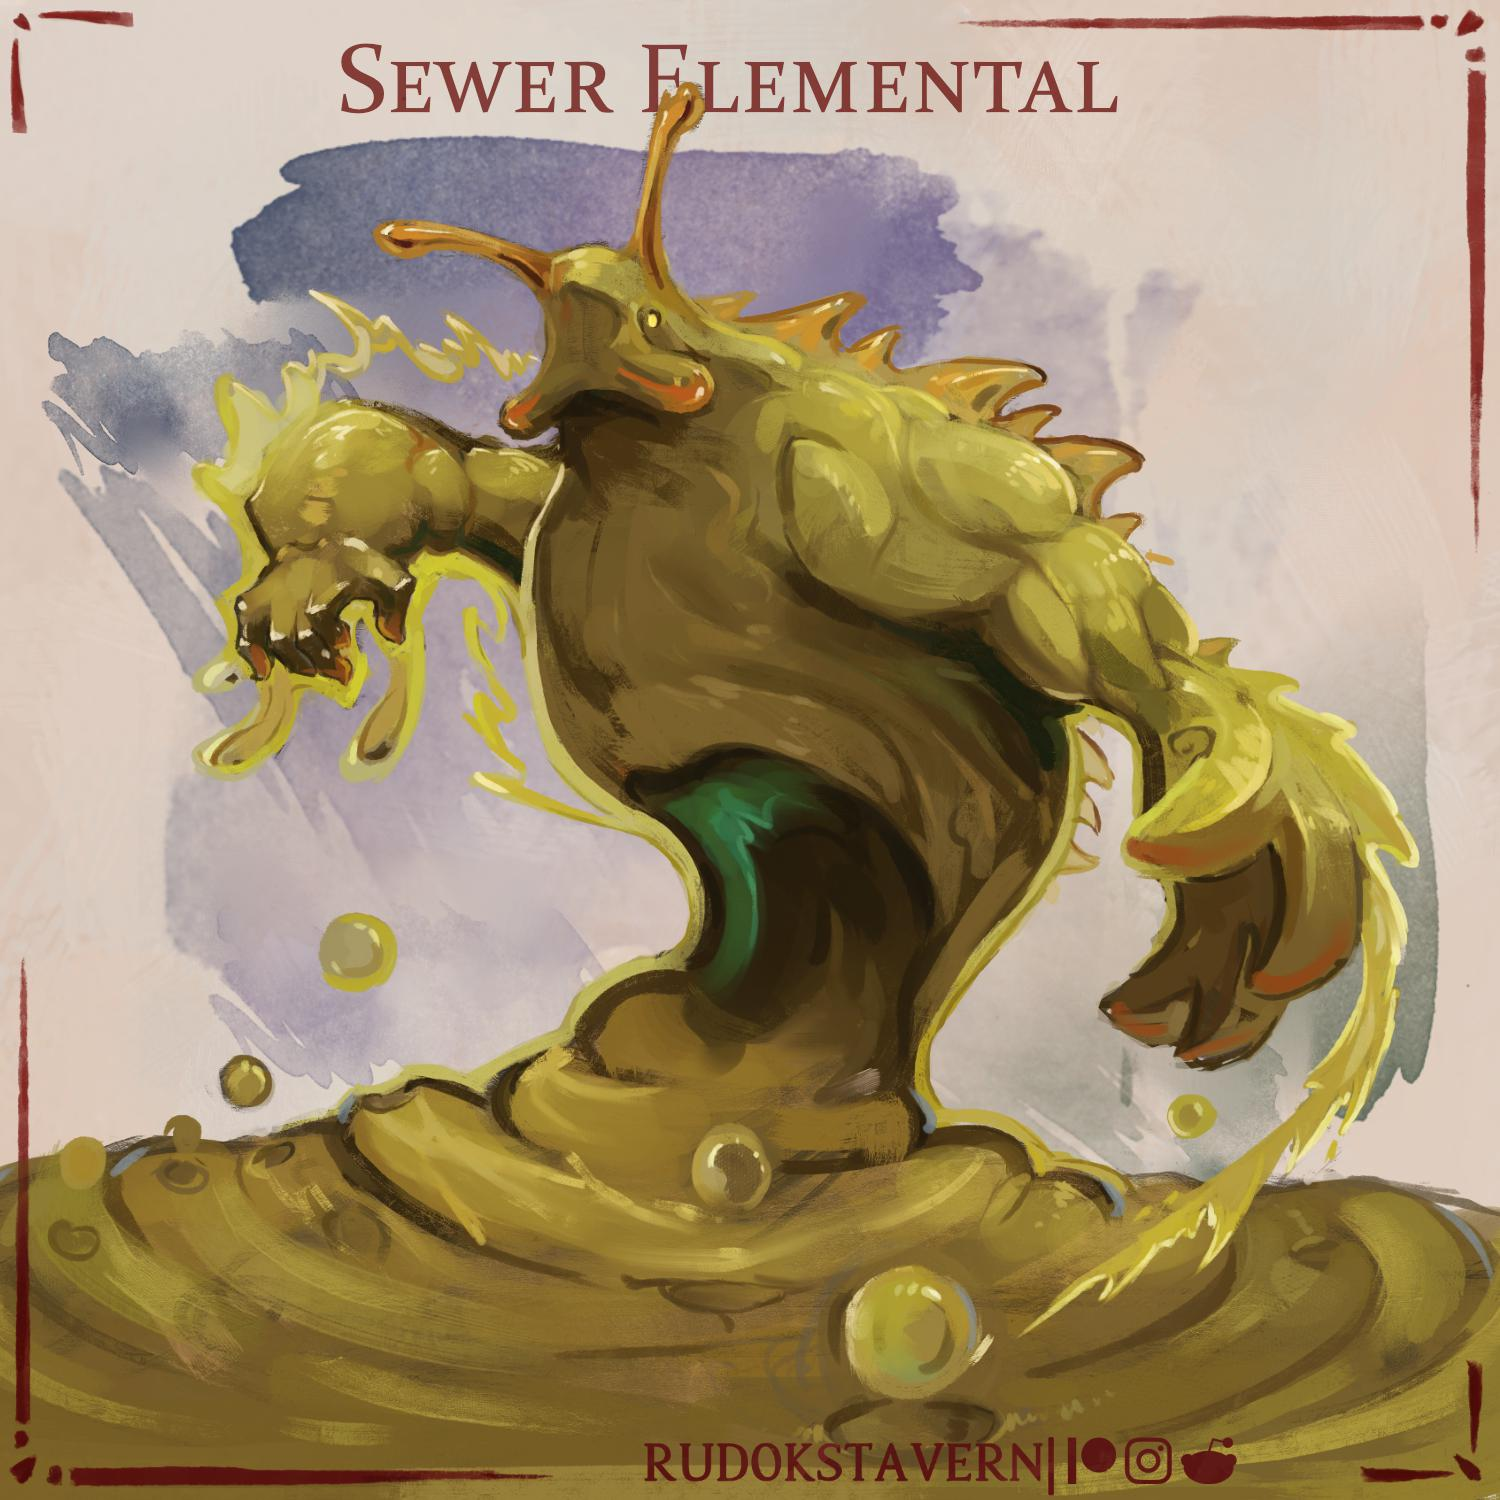
\includegraphics{6pnf9gio0d891.jpg}
\caption{6pnf9gio0d891.jpg}
\end{figure}

Informazioni Generali

Dimensione: Grande

Tipo: Costrutto?

Attitude:

Velocità di movimento: 30ft

Habitat: Fogne

Alleati:

Nemesi:

\begin{center}\rule{0.5\linewidth}{0.5pt}\end{center}

\subsection{1. Descrizione Generale}\label{descrizione-generale}

\begin{center}\rule{0.5\linewidth}{0.5pt}\end{center}

\begin{figure}
\centering
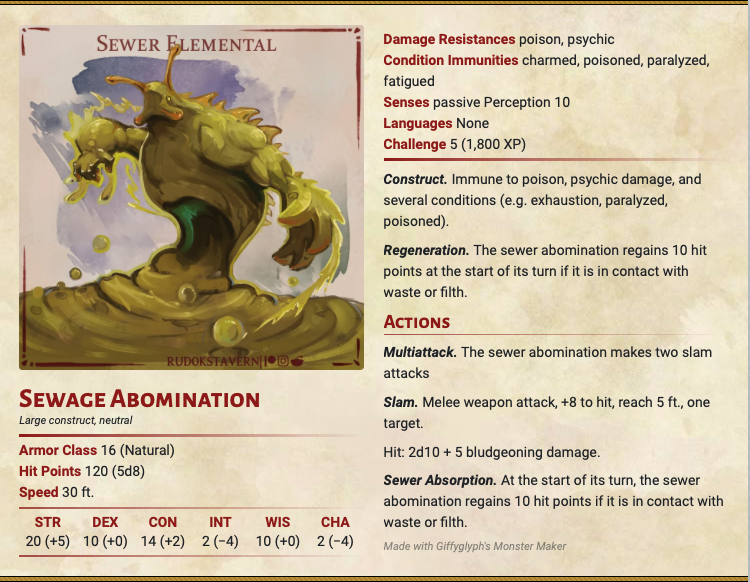
\includegraphics{Screen_Shot_2023-03-26_at_17.15.02_PM.png}
\caption{Screen Shot 2023-03-26 at 17.15.02 PM.png}
\end{figure}

A {[}monster{]}, sometimes called a {[}something{]} or {[}something
else{]} is normally found in {[}location{]}. Extremely {[}description{]}
and {[}description{]}, {[}monster{]} are considered {[}main info{]}.

{[}Monster{]} are easily identifiable because of their
{[}description{]}.

They are {[}slightly more detailed description{]}.

\begin{quote}
``blblblblbl''
\end{quote}

\subsection{2. Distribuzione e Habitat}\label{distribuzione-e-habitat}

\begin{center}\rule{0.5\linewidth}{0.5pt}\end{center}

{[}Monster{]} lives in {[}location{]}. It is sometimes found in
{[}another location{]}.

\subsection{3. Comportamento}\label{comportamento}

\begin{center}\rule{0.5\linewidth}{0.5pt}\end{center}

Info sul comportamento

\subsection{4. Variazioni}\label{variazioni}

\begin{center}\rule{0.5\linewidth}{0.5pt}\end{center}

Sono note varianti di questa creatura?

\subsection{5. Interazioni con gli
Umani}\label{interazioni-con-gli-umani}

\begin{center}\rule{0.5\linewidth}{0.5pt}\end{center}

Quali sono le interazioni che questa creatura ha/ha avuto con gli umani?

\subsubsection{5.1 {[}Creatura{]} nel
Folklore}\label{creatura-nel-folklore}

\begin{center}\rule{0.5\linewidth}{0.5pt}\end{center}

descrizione folkloristica

\subsection{6. Individui noti}\label{individui-noti}

\begin{center}\rule{0.5\linewidth}{0.5pt}\end{center}

Quali individui di questa creatura sono noti al grande pubblico?
